\documentclass{beamer}

\usepackage[utf8]{inputenc}
\usepackage[spanish]{babel}
\usepackage{booktabs, makecell, multirow}
\usepackage{graphicx}
\usepackage{tikz}
\usepackage{color, colortbl}
\usepackage[font=tiny,labelfont=bf, format=plain,justification=centering,labelformat=empty]{caption}
\usepackage{fontawesome6}
\usepackage{verbatim}
\usepackage{listings}
\lstset{basicstyle=\ttfamily\footnotesize, language=Bash}
\graphicspath{{./figures}}
\usetheme{CambridgeUS}

\renewcommand\theadfont{\bfseries} % bold tabular headers
\renewcommand\theadalign{ll}
\renewcommand\theadgape{}


\definecolor{mygray}{RGB}{100, 100, 100}
\definecolor{myred}{RGB}{175, 7, 31}
\setbeamercolor{palette primary}{bg=mygray,fg=myred}
\setbeamercolor{palette secondary}{bg=mygray!10!white,fg=myred}
\setbeamercolor{palette tertiary}{bg=myred,fg=white}
\setbeamercolor{block title}{bg=mygray, fg=black}
\setbeamercolor{block title alerted}{bg=myred, fg=white}
\setbeamercolor{block body}{fg=black,bg=mygray!10!white}
\setbeamercolor{block body alerted}{fg=black, bg=myred!10!white}
\setbeamerfont{block body}{size=\small}
\setbeamerfont{block body alerted}{size=\small}
\setbeamerfont{block body example}{size=\small}
\setbeamerfont{block title}{size=\small}
\setbeamerfont{block title alerted}{size=\small}
\setbeamerfont{block title example}{size=\small}
\hypersetup{
  colorlinks,
  allcolors=red,
  urlcolor=blue,
}
\setbeamercolor{section number projected}{bg=mygray,fg=myred}
\setbeamertemplate{itemize item}[triangle]
\setbeamercolor{itemize item}{fg=mygray}
\setbeamertemplate{itemize subitem}[circle]
\setbeamercolor{itemize subitem}{fg=myred!50!white}
\setbeamercolor{section in head/foot}{bg=myred!20!white, fg=mygray}


\title{Curso de Introducción a Git y GitHub}
\subtitle{Día 3 - Ramas y Código colaborativo}

\author{Héctor Nieto}

\institute{Instituto de Ciencias Agrarias, CSIC}
\date{2026}


\logo{
\includegraphics[height=0.5cm]{CSIC}}

\begin{document}

 \begin{frame}
  \titlepage
 \end{frame}

	\begin{frame}{Ramas}
	 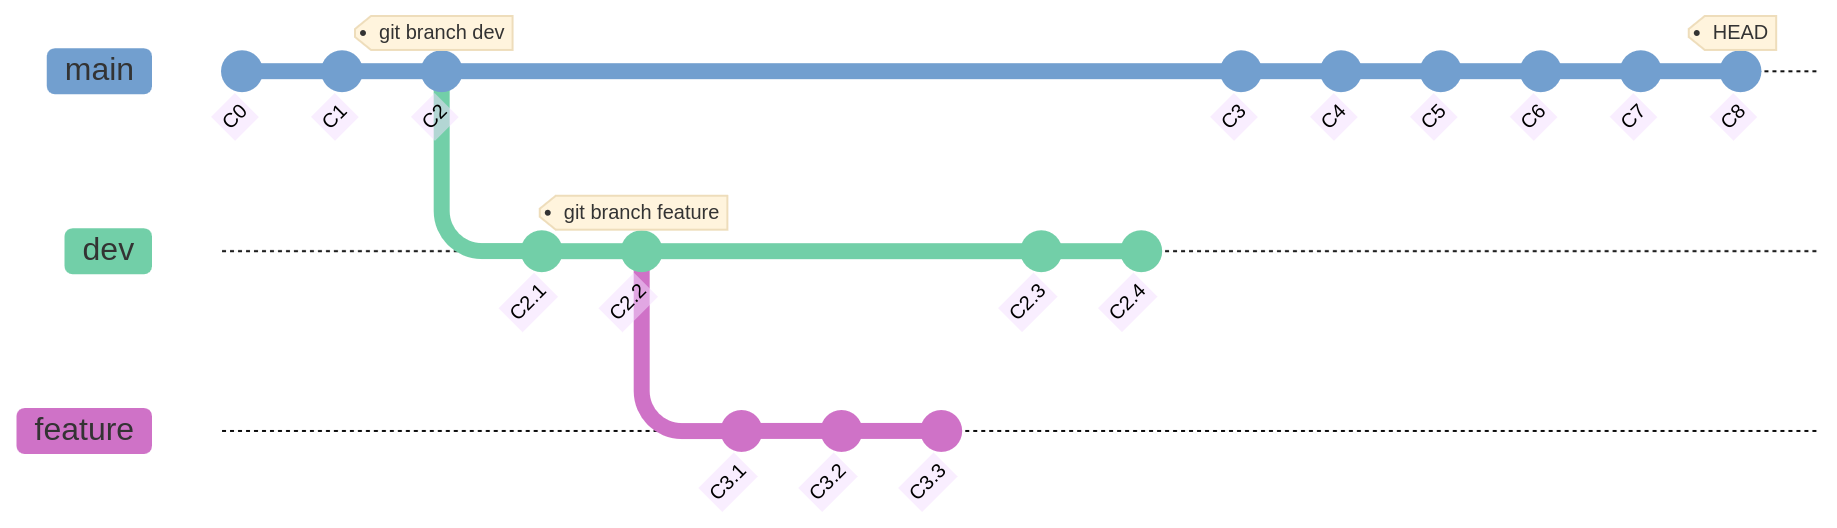
\includegraphics[width=\columnwidth]{03_git_branches}
	\end{frame}


	\begin{frame}{Fusionado: rebase}
	 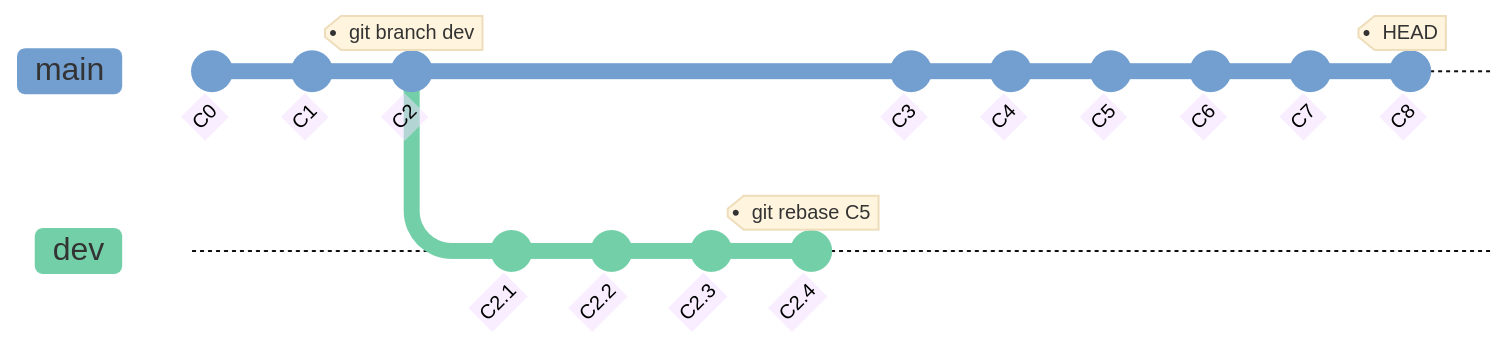
\includegraphics[width=\columnwidth]{03_git_rebase1}
	\end{frame}


	\begin{frame}{Fusionado: rebase}
	 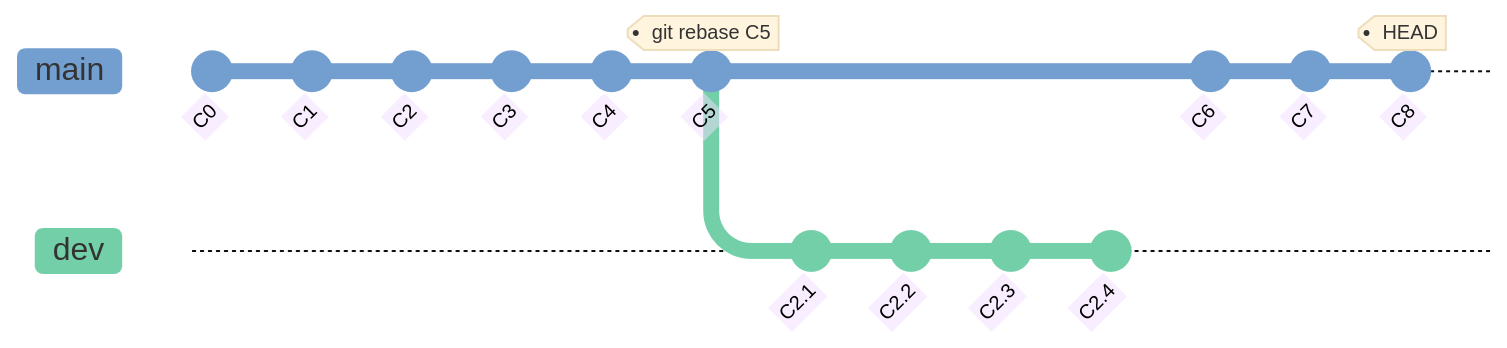
\includegraphics[width=\columnwidth]{03_git_rebase2}
	\end{frame}


	\begin{frame}{Fusionado: merge}
	 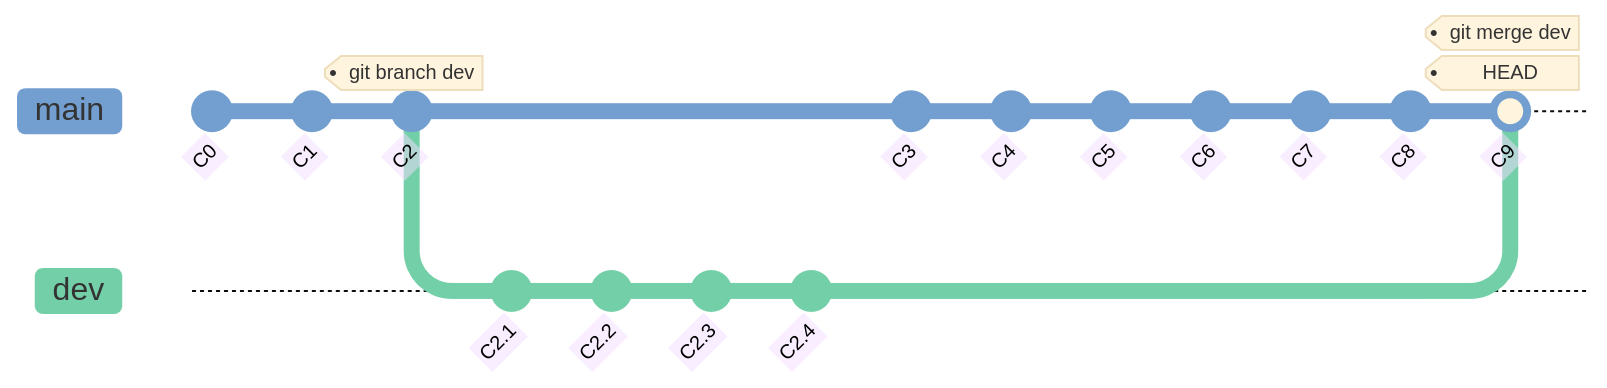
\includegraphics[width=\columnwidth]{03_git_merge1}
	\end{frame}


	\begin{frame}{Fusionado: merge}
	 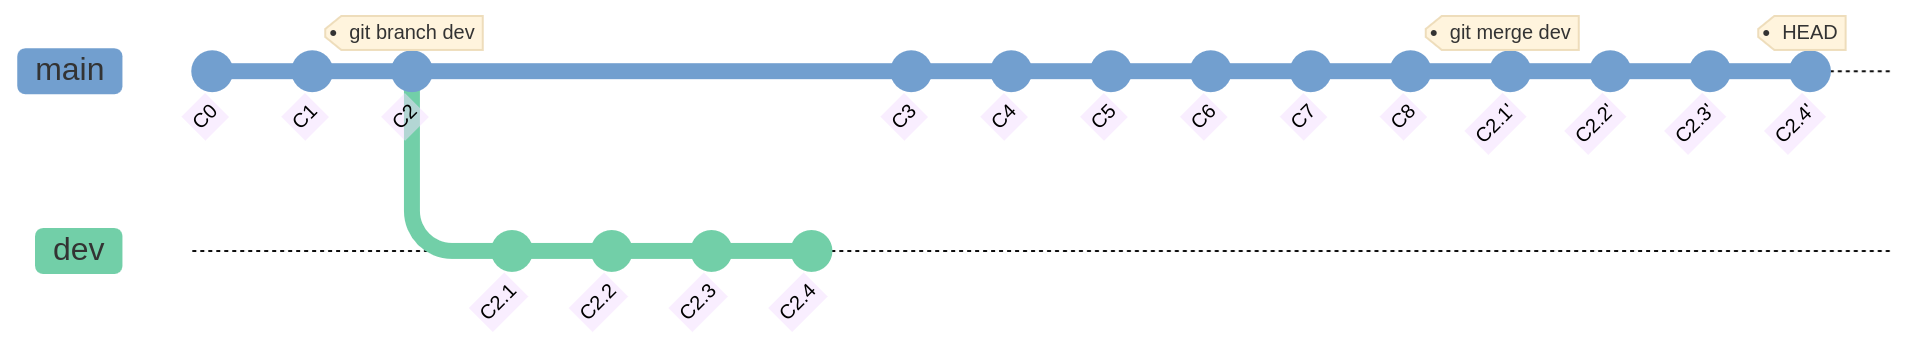
\includegraphics[width=\columnwidth]{03_git_merge2}
	\end{frame}

	\begin{frame}{Fusionado: resolución de conflictos}
	 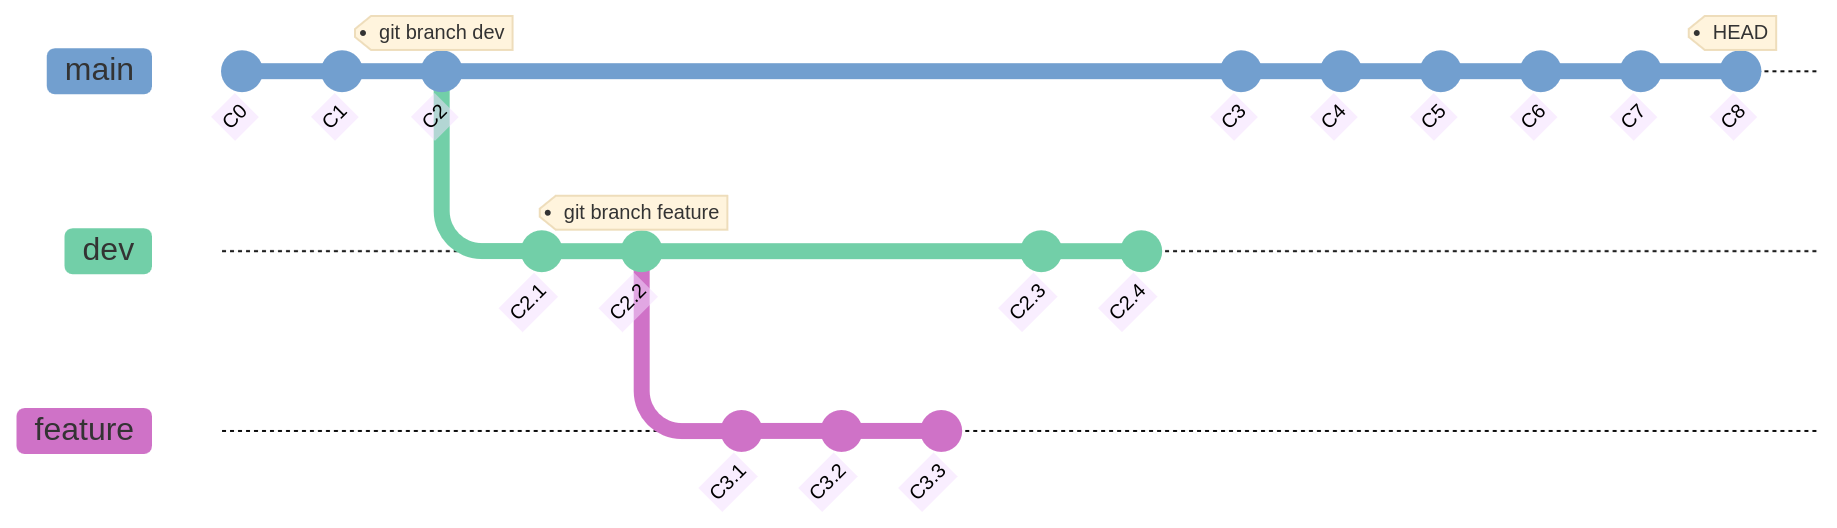
\includegraphics[width=\columnwidth]{03_git_branches}
  \begin{columns}
   \begin{column}{0.5\linewidth}
    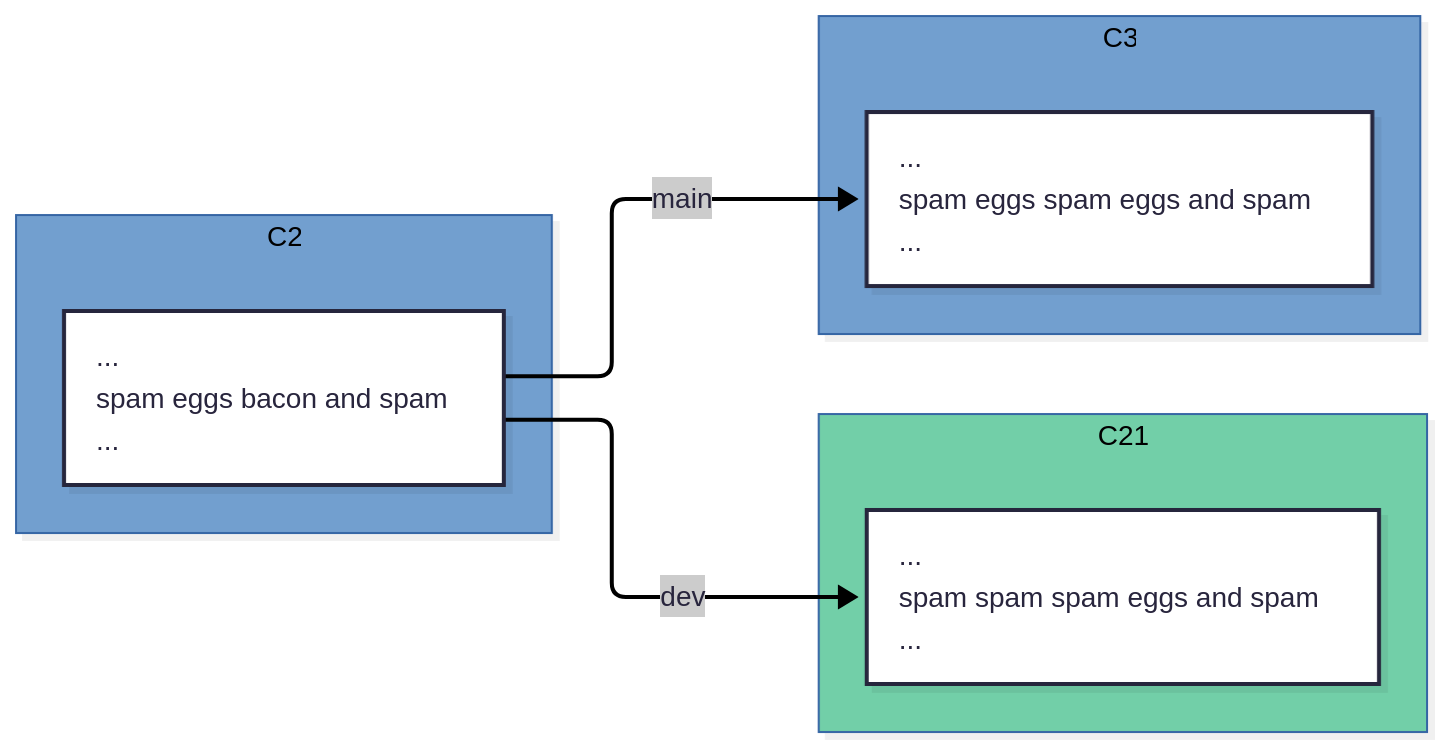
\includegraphics[height=0.4\textheight]{03_conflict1}
   \end{column}
			\begin{column}{0.3\linewidth}
    \Huge \faQuestion
   \end{column}
  \end{columns}
	\end{frame}


	\begin{frame}[fragile]{Fusionado: resolución de conflictos}
	\scriptsize
	 \begin{verbatim}
eggs and bacon
eggs sausage and bacon
eggs and spam
eggs bacon and spam
eggs bacon sausage and spam
spam bacon sausage and spam
spam eggs spam spam spam bacon and spam
>>>>>>>>HEAD
spam eggs spam eggs and spam
========
spam spam spam eggs and spam
<<<<<<<<C21
spam spam spam spam spam spam baked beans spam spam spam spam and spam
lobster termidor aux crevettes with a mornay sauce garnished with truffle pate, brandy and a fried egg on top and spam
	 \end{verbatim}
	\end{frame}


	\begin{frame}{Fusionado: resolución de conflictos}
	 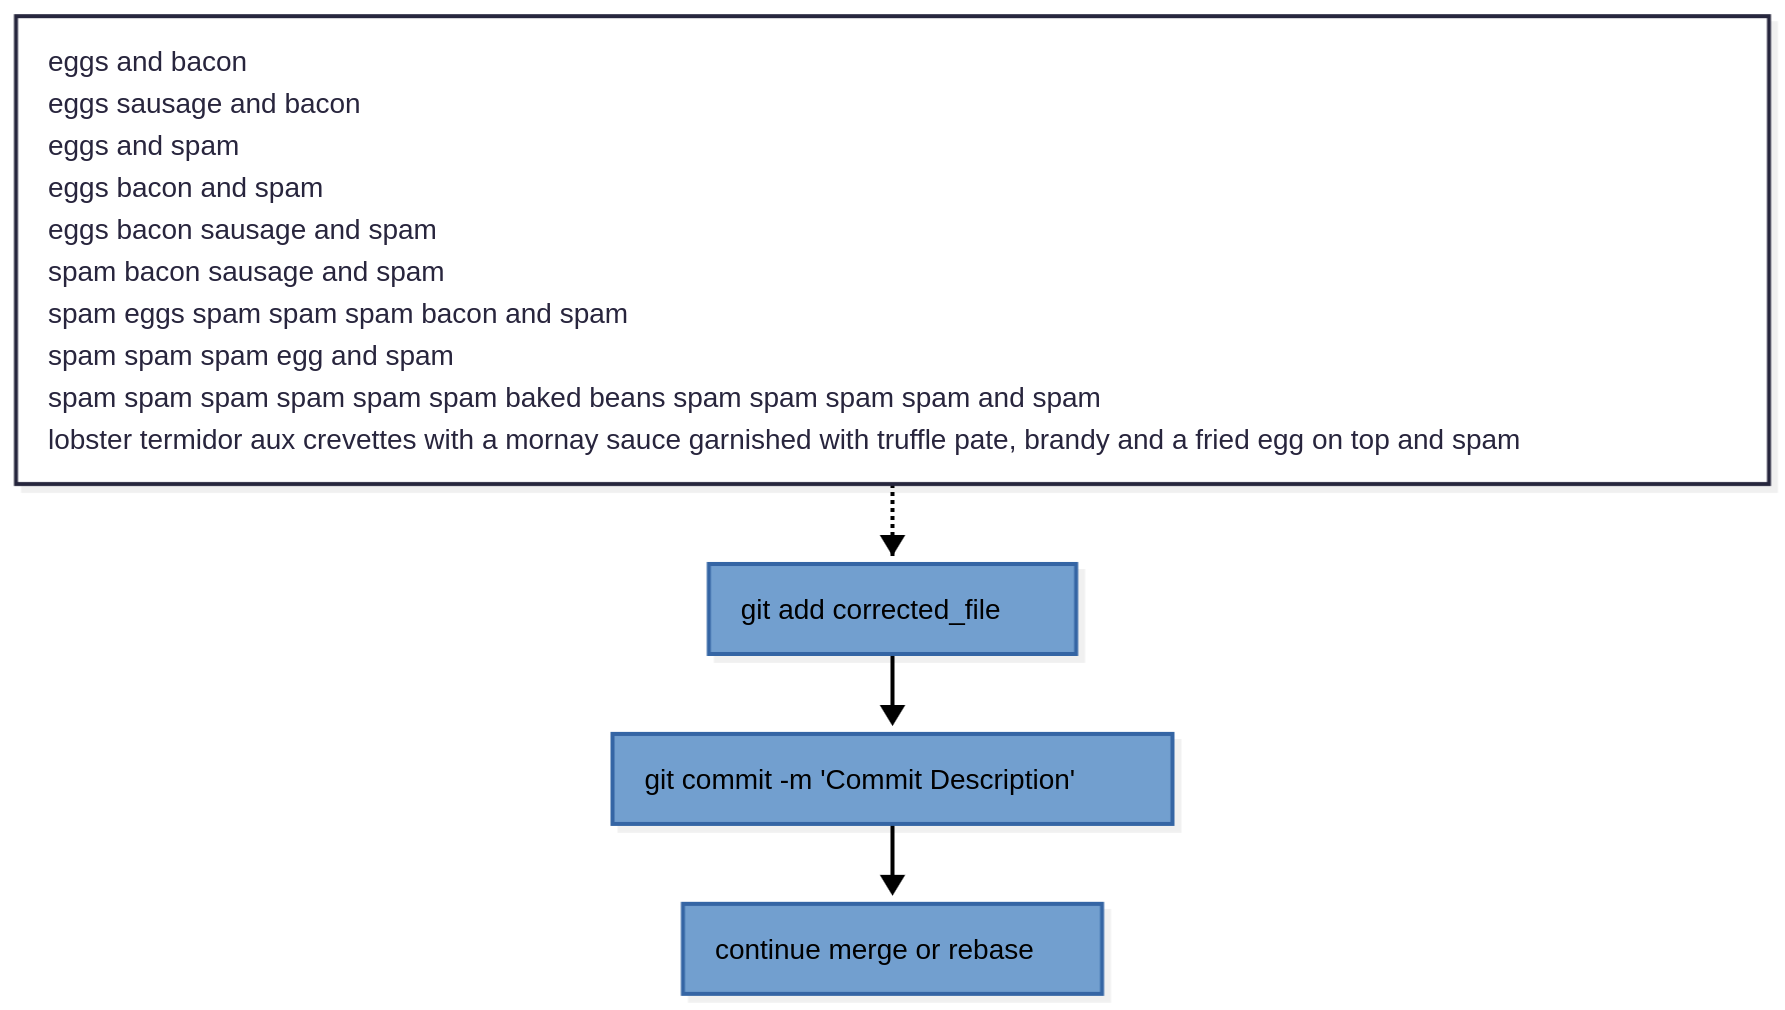
\includegraphics[height=0.8\textheight]{03_conflict2}
	\end{frame}


	\begin{frame}{Código colaborativo}
	 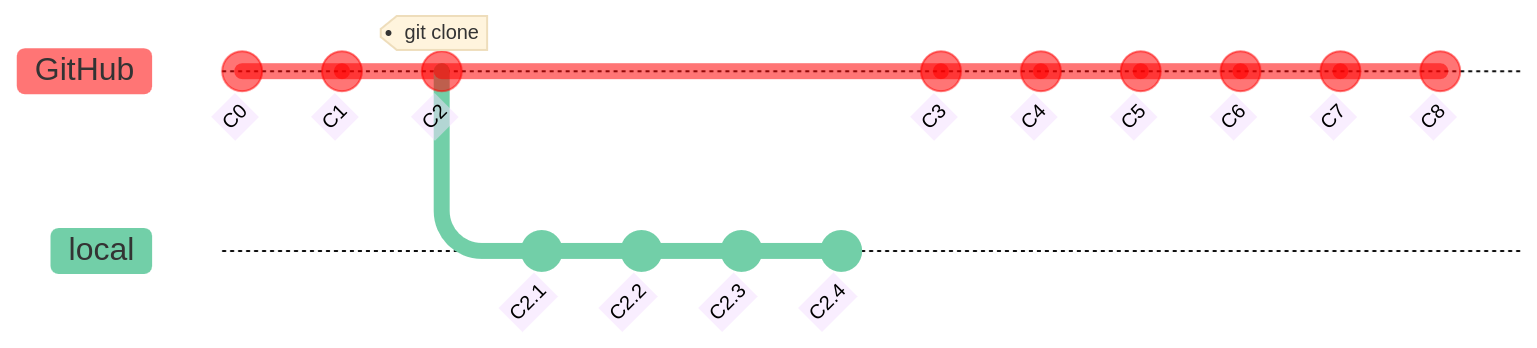
\includegraphics[width=\textwidth]{03_colaborative1}\\
	 Fork repository in GitHub
	 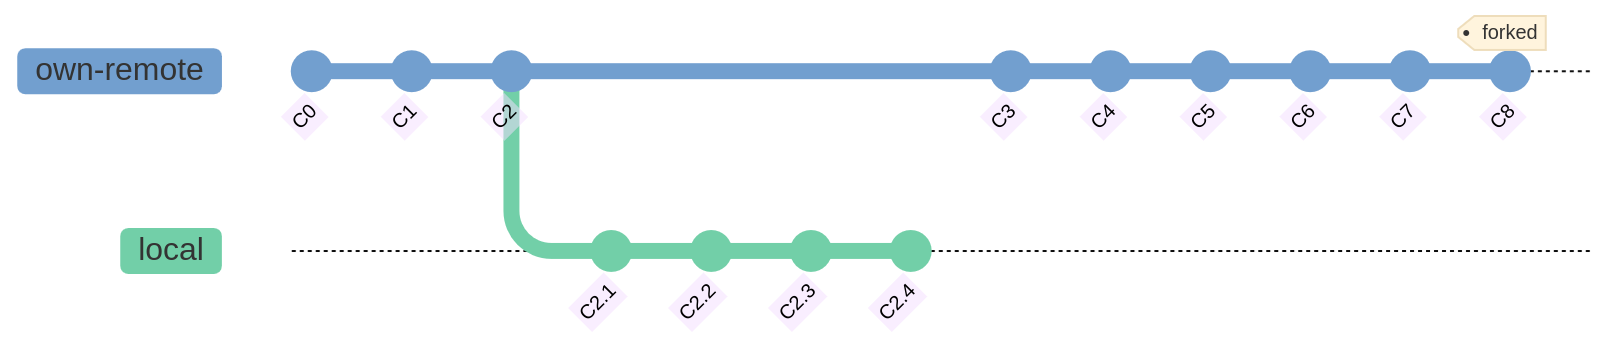
\includegraphics[width=\textwidth]{03_colaborative2}
	\end{frame}


	\begin{frame}{Código colaborativo}
	 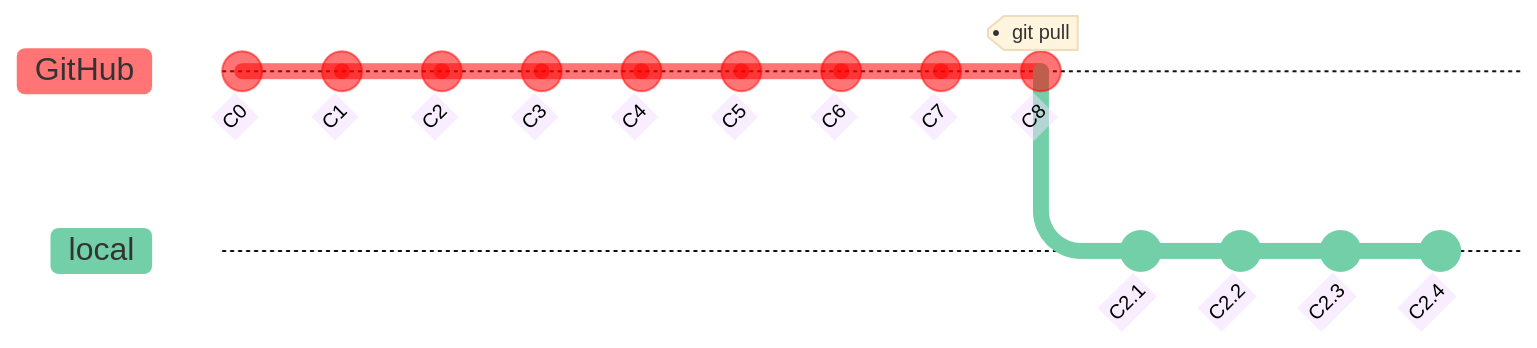
\includegraphics[width=\textwidth]{03_colaborative3}\\
	 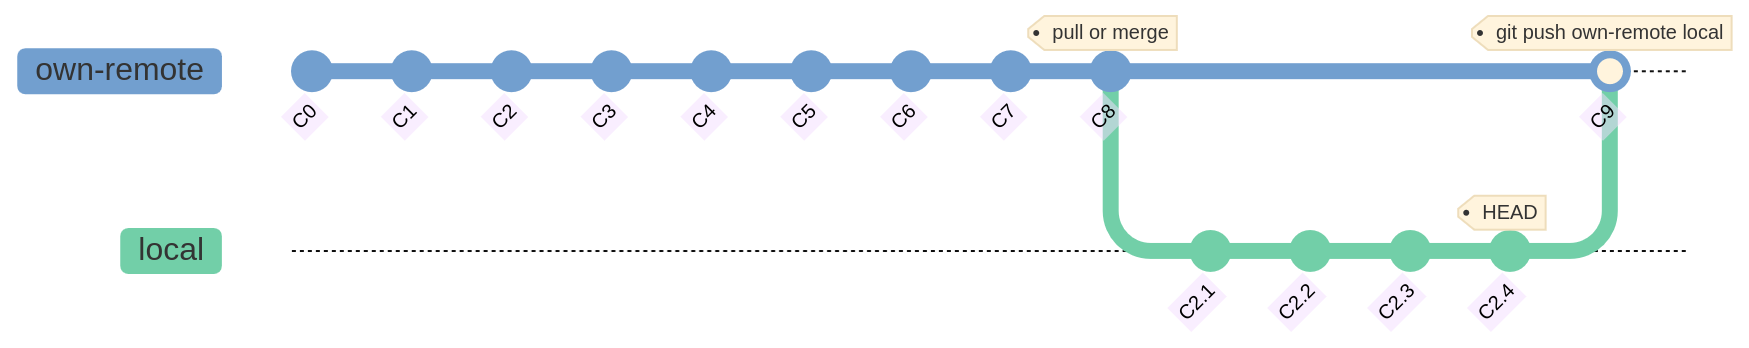
\includegraphics[width=\textwidth]{03_colaborative4}\\
	 Pull Request in GitHub
	\end{frame}


\end{document}
